 \documentclass[a4paper,10pt]{article}
\input{/Users/WannaGetHigh/workspace/latex/macros.tex}

\title{VisA : TP - Approche de la logique floue}
\author{Fran\c cois \bsc{Lepan}}

\begin{document}
\maketitle

\section{Fonctions d'appartenance}

\subsection{Programme g\'en\'erant des ensembles flous d'un univers du discours associ\'e \`a une variable num\'erique Temp\'erature}
Afin de recr\'eer ces ensembles floues on va g\'en\'erer 3 vecteurs de taille 40 avec des valeurs allant de 0 \`a 1 (\emph{cf.}~Fig.~\ref{univers}).

\begin{Verbatim}[commandchars=\\\{\}]
\codeRed{function} basse = \codeBlue{getCourbeBasse()}
    basse(1,1:10) = 1;
    basse(1,11:19) = 2 - ((0.9:0.1) - (-1/10)*(11:19));
    basse(1,20:40) = 0;
\codeRed{endfunction}

\codeRed{function} moyenne = \codeBlue{getCourbeMoyenne()}
    moyenne(1,1:10) = 0;
    moyenne(1,11:20) = -1 + ((0.9:0.1) - (-1/10)*(11:20));
    moyenne(1,20:29) = 3 - ((0:0.9) - (-1/10)*(20:29));
    moyenne(1,30:40) = 0;
\codeRed{endfunction}

\codeRed{function} haute = \codeBlue{getCourbeHaute()}
    haute(1,1:20) = 0;
    haute(1,21:29) = -2 + ((0:0.9) - (-1/10)*(21:29));
    haute(1,30:40) = 1;
\codeRed{endfunction}
\end{Verbatim}

\begin{figure}[ht]
\begin{center}
	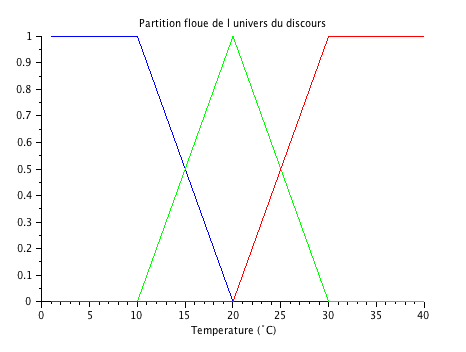
\includegraphics[width=7cm]{images/univers.png}
\end{center}
	\caption{Partition floue de l'univers du discours}
	\label{univers}
\end{figure}

\newpage

\subsection{Degr\'ee d'appartenance aux diff\'erents sous-ensembles pour une temp\'erature mesur\'ee de $16^oC$  }

\begin{Verbatim}[commandchars=\\\{\}]
temp_16_deg_basse = basse(16);
temp_16_deg_moyenne = moyenne(16);
temp_16_deg_haute = haute(16);

\codeBlue{//    affichage des degree d'appartenance}
    disp(temp_16_deg_basse);
    disp(temp_16_deg_moyenne);
    disp(temp_16_deg_haute);
\end{Verbatim}


\subsection{Graphique de la temp\'erature basse ou moyenne}

\begin{figure}[ht]
\begin{center}
	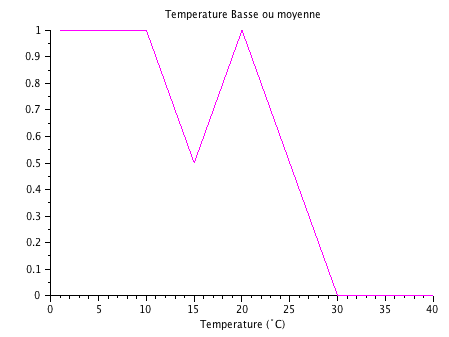
\includegraphics[width=7cm]{images/basse_ou_moyenne.png}
\end{center}
	\caption{Temperature basse ou moyenne}
	\label{basse_ou_moyenne}
\end{figure}

\section{Op\'erateurs de la logique floue}

\begin{Verbatim}[commandchars=\\\{\}]

\codeRed{function} minimum = \codeBlue{getSousEnsOperateurMin(a,b)}
    minimum = min(a,b);
\codeRed{endfunction}

\codeRed{function} maximum = \codeBlue{getSousEnsOperateurMax(a,b)}
    maximum = max(a,b);
\codeRed{endfunction}

\end{Verbatim}


\section{Implication floue}

Il faut tout d'abord r\'ecup\'erer les valeurs de la courbe \emph{chauffer fort} (\emph{cf.}~Fig.~\ref{chauffer_fort}). 

\begin{Verbatim}[commandchars=\\\{\}]
\codeRed{function} chauffeFort = \codeBlue{getCourbeChauffe()}
    chauffeFort(1,1:80) = 0;
    chauffeFort(1,81:99) = -0.3 + ((0.05:0.05:0.95) - (-1/300)*(81:99));
    chauffeFort(1,100:150) = 1;
\codeRed{endfunction}
\end{Verbatim}

\begin{figure}[ht]
\begin{center}
	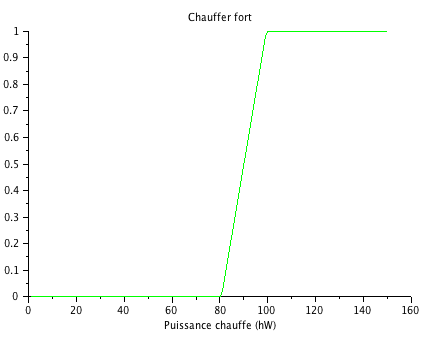
\includegraphics[width=7cm]{images/chauffer_fort.png}
\end{center}
	\caption{Chauffer fort}
	\label{chauffer_fort}
\end{figure}

\newpage

Ensuite il suffit de faire un \emph{min} entre un tableau de taille \'egale au tableau \emph{chauffeFort} avec la valeur du tableau \emph{basse(12)} c'est \`a dire le degr\'e d'appartenance de la courbe temp\'erature basse pour une temp\'erature \'egale \`a 12 degr\'e. \\

\begin{Verbatim}[commandchars=\\\{\}]
chauffeFort = getCourbeChauffe();

\codeBlue{// on creer un tableau de taille 15 avec la valeur se trouvant \`a basse(12) }
temp_mesure(1,1:150) = basse(12);

\codeBlue{// ensemble flou issue de l'utilisation de l'implication de Mamdani}
r = getSousEnsOperateurMin(temp_mesure,chauffeFort);
\end{Verbatim}
~\\

Et on obtient la ~Fig.~\ref{implication_floue}

\begin{figure}[ht]
\begin{center}
	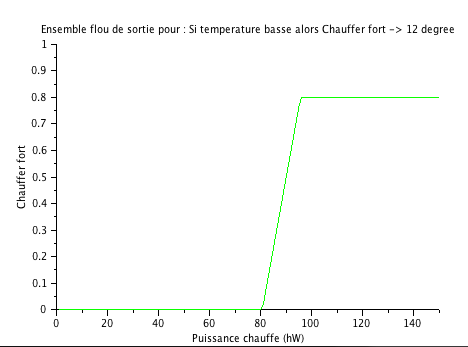
\includegraphics[width=6cm]{images/implication_floue.png}
\end{center}
	\caption{Implication floue pour }
	\label{implication_floue}
\end{figure}


\end{document}